\documentclass[../main.tex]{}
\begin{document}
We run our implementation of Clarke Wright saving algorithm and ruin and recreate algorithm on well-known CVRP testing benchmark data sets by without tuning any parameters. Clarke Wright saving algorithm does not give good solutions. It always yields solutions have large difference with best know solutions' value. However, ruin and recreate algorithm is very prominent. It produces solutions have difference best know values within 0\% - 10\% as table below:
\begin{table}[h]
\renewcommand{\arraystretch}{1.3}
\caption{Bench mark for instance B}
\label{tb:bnch_ins_b}
\centering
\begin{tabular}{|c|c|c|c|}
\hline
\bfseries Bench mark & \bfseries Best know value & \bfseries RR & \bfseries \% from optimal \\
\hline
B-n35-k5 & 955 & 985 & 3.14\%\\
B-n31-k5 & 672 & 701 & 4.32\%\\
B-n50-k7 & 741 & 784 & 5.80\%\\
B-n38-k6 & 805 & 854 & 6.09\%\\
B-n34-k5 & 788 & 838 & 6.35\%\\
\hline
\end{tabular}
\end{table}

\begin{table}[h]
\renewcommand{\arraystretch}{1.3}
\caption{Bench mark for instance E}
\label{tb:bnch_ins_e}
\centering
\begin{tabular}{|c|c|c|c|}
\hline
\bfseries Bench mark & \bfseries Best know value & \bfseries RR & \bfseries \% from optimal \\
\hline
E-n23-k3 & 569 & 570 & 0.18\%\\
E-n30-k3 & 534 & 540 & 1.12\%\\
E-n22-k4 & 375 & 393 & 4.80\%\\
E-n33-k4 & 835 & 888 & 6.35\%\\
E-n51-k5 & 521 & 656 & 25.91\%\\
\hline
\end{tabular}
\end{table}

\begin{figure}[!t]
\centering
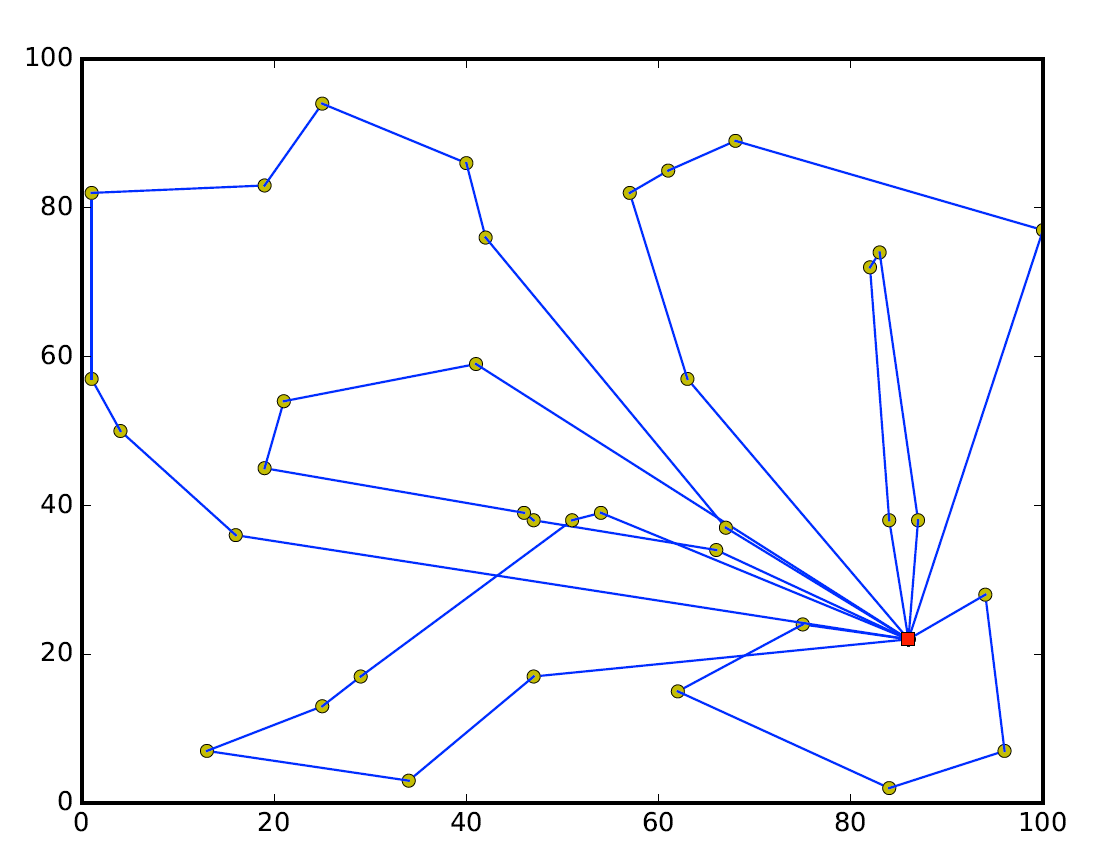
\includegraphics[width=2.5in]{A-n37-k6_952}
\caption{A solution for A-n37-k6 with cost 952}
\label{fig_sim}
\end{figure}

\end{document}